% Suggested time: 1.4 minutes
\begin{frame}[t]{OPD: dense feedback on student-generated states}
  \begin{columns}[T,onlytextwidth]
    \begin{column}{0.50\textwidth}
      \small
      \begin{enumerate}
        \item The student samples its own trajectory.
        \item An external teacher scores the next-token distribution at each student prefix.
        \item Reverse KL pulls the student toward the teacher on states the student actually visits.
      \end{enumerate}
    \end{column}
    \begin{column}{0.47\textwidth}
      \vspace{-2mm}
      \[
        P_t=\pi_\theta(\cdot\mid s_t),\qquad
        Q_t=\pi_T(\cdot\mid s_t)
      \]
      \vspace{-3mm}
      \[
        \mathcal L_{\mathrm{OPD}}=\sum_t D_{\mathrm{KL}}(P_t\|Q_t)
      \]

      \vspace{-2mm}
      \centering
      \begin{tikzpicture}[x=0.34cm,y=0.62cm]
        \begin{scope}[xshift=-1.75cm]
          \node[font=\tiny\bfseries] at (0,1.18) {Forward: covering};
          \draw[->,DeckMuted] (-2.25,0) -- (2.35,0);
          \draw[DeckInk,thick,domain=-2.15:2.15,samples=60,smooth]
            plot (\x,{0.82*exp(-((\x+1.0)^2)/0.16)+0.82*exp(-((\x-1.0)^2)/0.16)});
          \draw[DeckMuted,dashed,domain=-2.15:2.15,samples=60,smooth]
            plot (\x,{0.46*exp(-((\x-0.35)^2)/1.05)});
          \draw[DeckGold,very thick,domain=-2.15:2.15,samples=60,smooth]
            plot (\x,{0.46*exp(-((\x)^2)/2.2)});
        \end{scope}
        \begin{scope}[xshift=1.75cm]
          \node[font=\tiny\bfseries] at (0,1.18) {Reverse: seeking};
          \draw[->,DeckMuted] (-2.25,0) -- (2.35,0);
          \draw[DeckInk,thick,domain=-2.15:2.15,samples=60,smooth]
            plot (\x,{0.82*exp(-((\x+1.0)^2)/0.16)+0.82*exp(-((\x-1.0)^2)/0.16)});
          \draw[DeckMuted,dashed,domain=-2.15:2.15,samples=60,smooth]
            plot (\x,{0.46*exp(-((\x-0.35)^2)/1.05)});
          \draw[DeckTeal,very thick,domain=-2.15:2.15,samples=60,smooth]
            plot (\x,{0.79*exp(-((\x-1.0)^2)/0.17)});
        \end{scope}
      \end{tikzpicture}

      \vspace{-1mm}
      {\tiny black: teacher\quad dashed: initial\quad color: result}
    \end{column}
  \end{columns}

  \vspace{-1mm}
  {\centering
    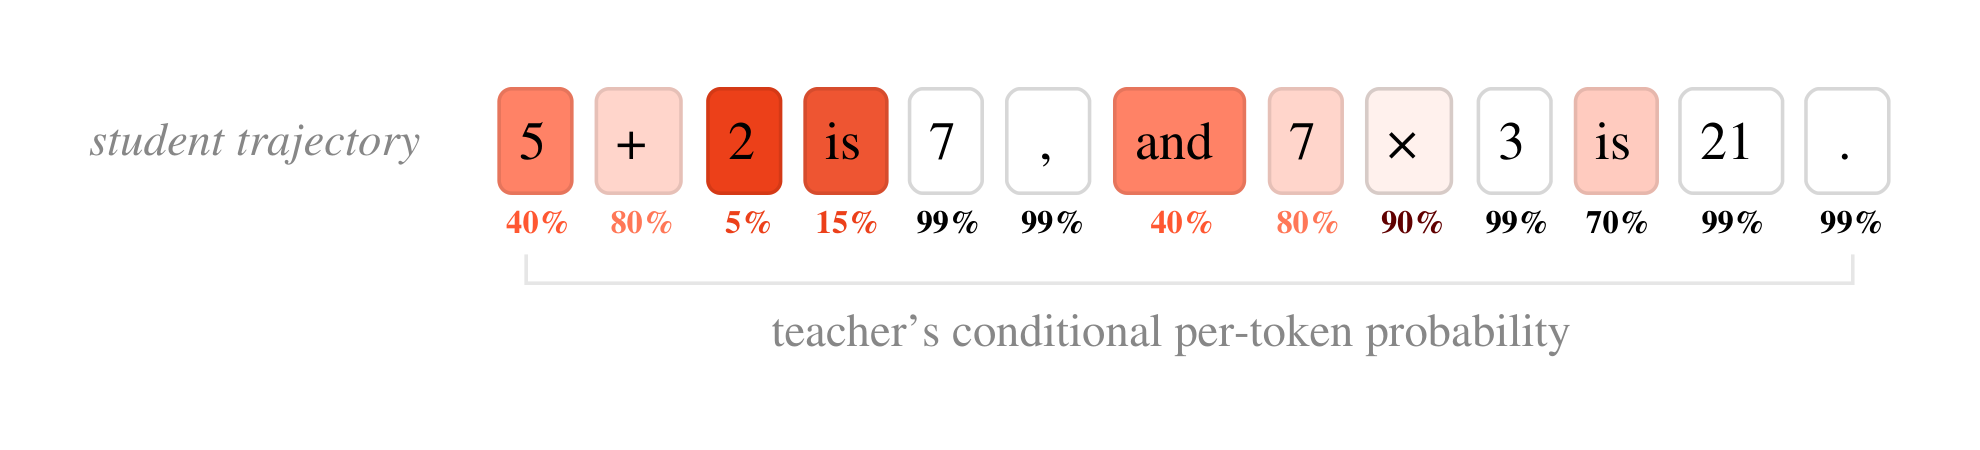
\includegraphics[width=0.65\textwidth]{figures/thinking_machines_opd_token_feedback.png}\par
    \vspace{-2mm}
    {\scriptsize Red tokens are locally unlikely under the teacher at the student's exact prefix
    \citep{agarwal2024onpolicy,lu2025onpolicydistillation}.}\par
  }
\end{frame}
